\documentclass[a4paper, 12pt]{article}
%\usepackage[utf8]{inputenc}
%\usepackage[vietnamese,english]{babel}
\usepackage[utf8]{vietnam}
\usepackage[margin = 2cm]{geometry}
\usepackage{graphicx}
\usepackage{amssymb}
\usepackage{amsthm}
\usepackage{amsmath}
\usepackage{xcolor}
\usepackage{nameref}
\usepackage{babel}
\usepackage{hyperref}
\usepackage{background}
\usepackage{graphics}
\usepackage{float}
\usepackage{enumerate}
\usepackage[]{enumitem}
\usepackage{indentfirst}
\setlength{\parindent}{0.5cm}

\usepackage{multicol}
\usepackage{multirow}
\usepackage{setspace}
\usepackage{array}
\onehalfspacing

% Cấu hình header và footer
\usepackage[]{fancyhdr}
\usepackage{titlesec}   % Để tạo sectioning tùy chỉnh
%\usepackage{chngcntr}   % Để reset counter
\usepackage{tocloft}
\fancyhf{}
\renewcommand{\thesection}{CHƯƠNG \arabic{section}.}
\renewcommand{\thesubsection}{\arabic{section}.\arabic{subsection}.}
\renewcommand{\thesubsubsection}{\arabic{section}.\arabic{subsection}.\arabic{subsubsection}.}

%\usepackage[backend=biber, style=ieee]{biblatex}
%\usepackage[style=ieee]{biblatex}
%\addbibresource{ref.bib} % Đường dẫn đúng đến tệp .bib

%% Định nghĩa counter trước
%\newcounter{subsubsubsection}[subsubsection]
%\renewcommand{\thesubsubsubsection}{\alph{subsubsubsection})}
%
%% Định nghĩa lệnh subsubsubsection
%\titleclass{\subsubsubsection}{straight}[\subsubsection]
%\titleformat{\subsubsubsection}[runin]
%{\normalfont\bfseries}
%{\thesubsubsubsection\ }
%{0pt}
%{}
%\titlespacing*{\subsubsubsection}{0pt}{3.25ex plus 1ex minus .2ex}{0.5em}
%
%% Thiết lập counter
%\counterwithin*{subsubsubsection}{subsubsection}

% Định nghĩa mục lục (sửa lỗi command đã tồn tại)
%\makeatletter
%\newcommand{\l@subsubsubsectioncustom}{\@dottedtocline{4}{4em}{2.3em}}
%\newcommand{\subsubsubsectionmark}[1]{
%	\addcontentsline{toc}{subsubsubsection}{\protect\numberline{\thesubsubsubsection}#1}
%}
%\makeatother

% Cấu hình mục lục
\renewcommand{\cftsecnumwidth}{8em} % Độ rộng cho "Chương X."
\renewcommand{\cftsubsecnumwidth}{4em} % Cho "X.Y."
\setlength{\cftsubsecindent}{2em} % Thụt lề subsection

%\fancyhead[R]{\texttt{GVHD: Nguyễn Trung Hiếu}}
%\fancyhead[R]{\thesection \leftmark}
%\fancyhead[L]{
\includegraphics[width=0.4\linewidth]{sections/pic/bk_name_en.png}}

%\fancyfoot[L]{
%%	
\includegraphics[height=12pt]{sections/pic/logo_DEE.png} \hspace{4pt}
%%	\textbf{Department of Electronics}%\\
%%%	\textit{EE3117/EE4451 – Digital IC Design Laboratory}
%	\texttt{SVTH: Nguyễn Đại Đồng - 2210780}
%}
\fancyfoot[R]{Page|\thepage}
\renewcommand{\headrulewidth}{0.4pt}
\renewcommand{\footrulewidth}{0.4pt}

% Cấu hình background
\backgroundsetup{
	scale=1,
	color=black,
	opacity=0.4,
	angle=0,
	contents={%
		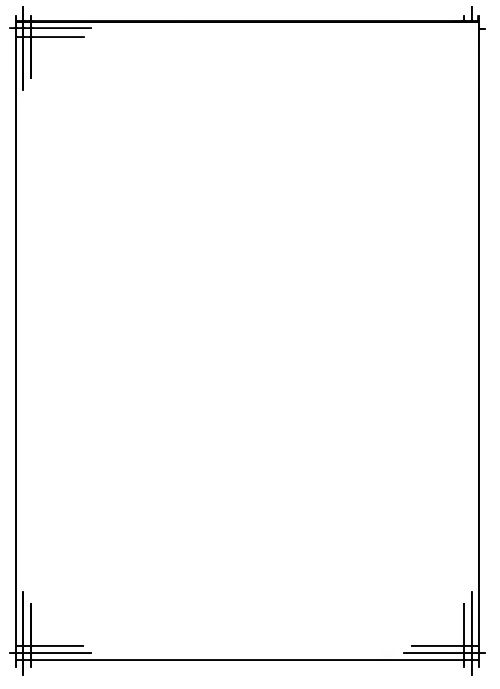
\includegraphics[width=\paperwidth,height=\paperheight]{sections/pic/bia.jpg}
	}
}


\usepackage{listings}

% Cấu hình màu sắc cho code
\definecolor{codegreen}{rgb}{0,0.6,0}
\definecolor{codegray}{rgb}{0.5,0.5,0.5}
\definecolor{codepurple}{rgb}{0.58,0,0.82}
\definecolor{backcolour}{rgb}{0.95,0.95,0.92}

% Định nghĩa style cho code
\lstdefinestyle{StyleCode}{
	backgroundcolor=\color{white},  % Màu nền trắng
	commentstyle=\color{codegreen},
	keywordstyle=\color{magenta},
	numberstyle=\tiny\color{codegray},
	stringstyle=\color{codepurple},
	basicstyle=\ttfamily\footnotesize,
	breakatwhitespace=false,
	breaklines=true,
	captionpos=b,
	keepspaces=true,
	numbers=left,
	numbersep=9pt,
	showspaces=false,
	showstringspaces=false,
	showtabs=false,
	tabsize=3,
	frame=single,                  % Khung đơn bao quanh code
	rulecolor=\color{black},       % Màu khung (đen)
	framexleftmargin=5pt,          % Khoảng cách lề trái khung
	framexrightmargin=5pt,         % Khoảng cách lề phải khung
	framextopmargin=3pt,           % Khoảng cách lề trên khung
	framexbottommargin=3pt         % Khoảng cách lề dưới khung
}
% Định nghĩa ngôn ngữ cho C
\lstdefinelanguage{C}{
	keywords={break, case, char, const, continue, default, do, double, else, enum, extern, float, for, goto, if, int, long, register, return, short, signed, sizeof, static, struct, switch, typedef, union, unsigned, void, volatile, while},
	sensitive=true,
	comment=[l]{//},
	morecomment=[s]{/*}{*/},
	morestring=[b]",
	morestring=[b]'
}
% Định nghĩa ngôn ngữ cho SystemVerilog
\lstdefinelanguage{SystemVerilog}{
	keywords={module, endmodule, input, output, wire, reg, logic, always, assign, begin, end, if, else, case, default, for, while, repeat, forever, fork, join, initial, task, function, return, break, continue, typedef, struct, enum, union, package, import, export, parameter, localparam, defparam, generate, endgenerate, always_comb, always_ff, always_latch, posedge, negedge, edge, wait, assert, assume, cover, property, sequence, rand, randc, constraint, randomize, with, inside, dist, class, endclass, extends, virtual, interface, endinterface, clocking, endclocking, modport, covergroup, endgroup, forkjoin, unique, priority, casex, casez, packed, unsigned, signed, static, automatic, protected, local, const, ref, this, super, new, null, extern, pure, forkjoin_none, time, bit, byte, shortint, int, longint, integer, time, real, shortreal, chandle, string, event, void, null, input, output, inout, tri, triand, trior, tri0, tri1, supply0, supply1, wand, wor, weak0, weak1, pullup, pulldown, highz0, highz1, small, medium, large, scalared, vectored},
	sensitive=true,
	morecomment=[l]//,
	morecomment=[s]{/*}{*/},
	morestring=[b]",
	morestring=[b]'
}

% Định nghĩa style cho result
\lstdefinestyle{StyleResult}{
	backgroundcolor=\color{backcolour},
	commentstyle=\color{codegreen},
	keywordstyle=\color{magenta},
	numberstyle=\tiny\color{codegray},
	stringstyle=\color{codepurple},
	basicstyle=\ttfamily\footnotesize,
	breakatwhitespace=false,
	breaklines=true,
	captionpos=b,
	keepspaces=true,
	numbers=none,
	numbersep=5pt,
	showspaces=false,
	showstringspaces=false,
	showtabs=false,
	tabsize=2,
	language=Result
}
% Định nghĩa cho thêm result
\lstdefinelanguage{Result}{
	keywords={PASS, FAIL, Time, TestCase},
	sensitive=true
}

\begin{document}
	\pagestyle{empty}
	\BgThispage
\begin{center}
	\Large\textbf{ĐẠI HỌC QUỐC GIA TP.HỒ CHÍ MINH \\ TRƯỜNG ĐẠI HỌC BÁCH KHOA\\ KHOA ĐIỆN - ĐIỆN TỬ \\ BỘ MÔN ĐIỆN TỬ \\--oo0oo--}
\end{center}
\vspace{0.4cm}
\begin{center}
	
\includegraphics[width=0.3\linewidth]{sections/pic/01_logobachkhoatoi.png}
\end{center}
\vspace{0.4cm}
\begin{center}
	\LARGE\textbf{BÁO CÁO ĐỒ ÁN 1}
	\vspace{0.1cm}
	
	\Large{Design and Implementation of a Power-Efficient Viterbi
		Encoding and Decoding Architecture on FPGA: From
		Theory to Practical Application}
\end{center}
\vspace{1cm}

\LARGE

\hspace{2cm}\begin{tabular}{p{0.4\linewidth} p{0.5\linewidth}}
	Giảng viên hướng dẫn: & Nguyễn Trung Hiếu\\
	Sinh viên thực hiện:  & Nguyễn Đại Đồng \\
	Mã số sinh viên:      & 2210780
\end{tabular}

\vspace{5cm}
\begin{center}
	\fontsize{8pt}{5pt}\selectfont\textbf{Tp.HCM, \dots/\dots/20\dots}
\end{center}

\newpage
\pagestyle{fancy}
\fontsize{13}{14}\selectfont
\fancyhead[L]{Lời cảm ơn}
\fancyhead[R]{GVHD: Nguyễn Trung Hiếu}
\section*{\centering LỜI CẢM ƠN}

Trước tiên, tôi xin gửi lời cảm ơn chân thành đến các thầy cô trong khoa Điện tử - Viễn thông, những người đã tận tình giảng dạy, truyền đạt kiến thức và kinh nghiệm quý báu trong suốt quá trình học tập, giúp tôi có nền tảng vững chắc để thực hiện đồ án này. Đặc biệt, tôi xin bày tỏ lòng biết ơn sâu sắc đến thầy Nguyễn Trung Hiếu, người đã trực tiếp hướng dẫn, hỗ trợ và định hướng tôi trong suốt quá trình nghiên cứu và hoàn thiện đồ án. Những góp ý quý giá và sự động viên của thầy đã giúp tôi vượt qua nhiều khó khăn và hoàn thành công việc một cách tốt nhất.

Tôi cũng xin gửi lời cảm ơn đến gia đình, bạn bè và các đồng nghiệp đã luôn ủng hộ, động viên và chia sẻ cùng tôi trong suốt quá trình thực hiện. Sự hỗ trợ về tinh thần lẫn vật chất từ mọi người là nguồn động lực lớn lao để tôi hoàn thành đồ án này.

Cuối cùng, tôi xin cảm ơn các tài liệu tham khảo, nguồn thông tin từ sách, báo, và các công cụ mô phỏng như ngôn ngữ lập trình C và SystemVerilog, đã cung cấp nền tảng lý thuyết và thực tiễn để tôi triển khai thành công nội dung đồ án. Mặc dù đã cố gắng hết sức, đồ án vẫn có thể còn những thiếu sót, tôi rất mong nhận được những ý kiến đóng góp để hoàn thiện hơn.

Trân trọng,

\vspace{6cm}
\hspace{6cm} \textit{Tp. Hồ Chí Minh, ngày \dots tháng \dots năm \dots }

\hspace{10cm} \textbf{Sinh viên}

\newpage
\fancyhead[L]{Đồ án môn học}
\section*{\centering TÓM TẮT ĐỒ ÁN}

Đồ án này trình bày về quá trình nghiên cứu, thiết kế và mô phỏng thuật toán giải mã Viterbi trong hệ thống truyền thông số, tập trung vào mã hóa và giải mã kênh sử dụng mã chập (Convolutional Codes). Nội dung bao gồm cơ sở lý thuyết về mã hóa kênh truyền, cấu trúc bộ mã hóa chập, và nguyên lý hoạt động của thuật toán Viterbi, một phương pháp giải mã tối ưu dựa trên quy hoạch động. Đồ án mô phỏng thuật toán Viterbi bằng ngôn ngữ lập trình C và SystemVerilog, với việc triển khai các khối chức năng như Branch Metric Unit (BMU), Add Compare Select Unit (ACSU) và Survivor Path Memory Unit (SPMU). Kết quả mô phỏng cho thấy khả năng khôi phục chính xác chuỗi bit gốc từ tín hiệu bị nhiễu, với ví dụ cụ thể sử dụng bộ mã hóa chập (3,1,2) và chuỗi đầu vào “110110”. Đồ án không chỉ cung cấp cái nhìn sâu sắc về kỹ thuật mã hóa và giải mã mà còn chứng minh tính hiệu quả của thuật toán Viterbi trong việc cải thiện độ tin cậy của hệ thống truyền thông.

\newpage
\tableofcontents
\listoffigures
\listoftables
	\pagestyle{fancy}
	\fontsize{13}{14}\selectfont
	%\section{Cơ sở lý thuyết}
\section{CỞ SỞ LÝ THUYẾT}

\subsection{Mã hóa kênh truyền trong lĩnh vực truyền thông thông tin}

\begin{figure}[H]
	\centering
	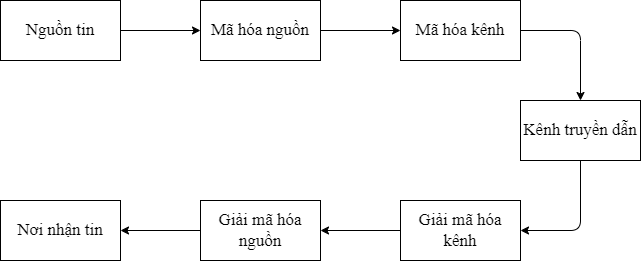
\includegraphics[width=0.6\linewidth]{sections/pic/cosolythuyet/ma-hoa-kenh.png}
	\caption{Mô hình hệ thống truyền thông số.}
	\label{f_mo-hinh-he-thong-truyen-thong-so}
\end{figure}

Mã hóa kênh truyền (Channel Coding) là một khâu quan trọng trong hệ thống truyền thông tin cùng với khối mã hóa nguồn. Mã hóa kênh là kỹ thuật thêm thông tin dư thừa (redundant information) vào tín hiệu gốc trước khi truyền để phát hiện và/hoặc sửa lỗi trong quá trình truyền qua kênh nhiễu.

Ở hình \ref{f_mo-hinh-he-thong-truyen-thong-so} thể hiện hệ thống truyền thông đơn giản trong đó,
\begin{itemize}[label=-]
	\item Nguồn tin: là nơi tạo ra thông tin cần truyền đi hay là thông tin mong muốn truyền.
	\item Mã hóa nguồn: là bộ mã hóa cho phép loại bỏ những thông tin dư thừa của chuỗi đầu vào.
	\item Mã hóa kênh: là bộ mã hóa cho phép ghép thêm các thông tin dư thừa vào chuỗi đầu vào.
	\item Kênh truyền dẫn: là các phương thức truyền thông tin có thể là không dây hoặc là hữu tuyến, vệ tinh.
\end{itemize}

Việc thêm khối mã hóa kênh vào hệ thống truyền thông số là do thường tín hiệu trong truyền thông thực tế sẽ thường xảy ra các lỗi như: Lỗi ngầu nhiên (Random Errors) do nhiễu trắng Gaussian (AWGN), Lỗi theo cụm (Burst Errors) do fading đa đường hoặc mất gói dữ liệu trong truyền thông không dây. Vì vậy, cần thêm khối mã hóa kênh vào để giúp cải thiện tỷ lệ lỗi bit (BER - Bit Error Rate) mà không cần tăng công suất truyền, còn giúp đảm bảo tính toàn vẹn của dữ liệu trong truyền thông không dây, hữu tuyến, và vệ tinh.

Có các loại mã hóa kênh phổ biến là:
\begin{itemize}[label = -]
	\item Mã khối (Block Codes): Dữ liệu được chia thành các khối có độ dài cố định, và các bit dư thừa thêm vào mỗi khối. Ví dụ: Mã Hamming, Mã Reed-Solomon.
	\item Mã chập (Convolutional Codes): Dữ liệu được mã hóa liên tục thông qua một bộ mã hóa dựa vào các thanh ghi dịch và phép toán XOR. Đặc trưng bởi các tham số: Độ dài ràng buộc (Constraint length), Tỷ lệ mã hóa (Code rate).
	\item Mã Turbo (Turbo Codes): Kết hợp nhiều bộ mã hóa và sử dụng kỹ thuật lặp (Iterative decoding) để đạt hiệu suất gần với giới hạn lý thuyết.
	\item Mã LDPC (Low-Density Parity-Check Codes): Sử dụng ma trận kiểm tra chẵn lẻ (Parity-check matrix) thưa thớt để đạt hiệu suất cao.
\end{itemize}

\subsection{Mã hóa sử dụng Mã chập (Convolutional Encoder)}

\begin{figure}[H]
	\centering
	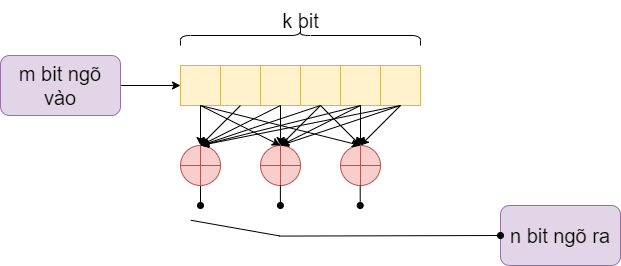
\includegraphics[width=.7\linewidth]{sections/pic/cosolythuyet/structure_convolutional_code.png}
	\caption{Cấu trúc tổng quát của một bộ mã hóa chập}
	\label{f_structure-convolutional-code}
\end{figure}

Mã chập được tạo ra bằng cách cho chuỗi thông tin truyền qua hệ thống các thanh ghi dịch tuyến tính có số trạng thái hữu hạn. Số lượng thanh ghi là \( K \), trong đó \( L = K + 1\) là \textbf{chiều dài ràng buộc} (constraint length). Bộ mã hóa chập có \( m \) bit ngõ vào và \( n \) bit ngõ ra. Tốc độ mã là \( r = m/n \), là tỉ số giữa số bit ngõ vào và số bit ngõ ra của tín hiệu. Tham số \( K \) thể hiện số lượng bit đầu vào (bao gồm bit đầu vào hiện tại và các bit đầu vào trước đó được lưu trong thanh ghi) ảnh hưởng đến đầu ra.

Một bộ mã hóa chập có cấu trúc gồm các thanh ghi dịch và các bộ cộng modulo-2. Các thanh ghi dịch lưu trữ các bit đầu vào trước đó, và các bộ cộng modulo-2 kết hợp các bit đầu vào hiện tại với các bit trong thanh ghi để tạo ra các bit đầu ra. 

Giả sử, $u$ là vector đầu vào, $x$ là vector đầu ra tương ứng được mã hóa từ vector $u$, bây giờ chúng ta mô tả cách tạo ra $x$ từ $u$. Để mô tả bộ mã hóa chúng ra cần phải kết nối vector $u$ vào thanh ghi đầu vào và $x$ vào thanh ghi đầu ra trong hình \ref{f_structure-convolutional-code}. Để có thể tính toán một cách dễ dàng, chúng ta tiến hành mô hình hóa bộ mã ở hình \ref{f_structure-convolutional-code} thành một ma trận sinh $G$ có dạng :

\[
\mathbf{G} = 
\begin{bmatrix}
	g_{1,0} & g_{1,1} & g_{1,2} & \cdots & g_{1,K-1} \\
	g_{2,0} & g_{2,1} & g_{2,2} & \cdots & g_{2,K-1} \\
	\vdots & \vdots & \vdots & \ddots & \vdots \\
	g_{n,0} & g_{n,1} & g_{n,2} & \cdots & g_{n,K-1}
\end{bmatrix}
\]

Trong đó:
\begin{itemize}[label = -]
	\item \( g_{i,j} \): Hệ số kết hợp (0 hoặc 1) cho biết bit đầu vào thứ \( j \) có tham gia vào bit đầu ra thứ \( i \) hay không.
	\item \( g_{i,j} = 1 \): Bit đầu vào thứ \( j \) được sử dụng để tính bit đầu ra thứ \( i \).
	\item \( g_{i,j} = 0 \): Bit đầu vào thứ \( j \) không được sử dụng để tính bit đầu ra thứ \( i \).
\end{itemize}

Vậy để được vector $x$ thì ta chỉ cần thực hiện phép nhân ma trận $G$ và vector $u$ lại với nhau: 
\[ x = u \cdot G \]

Để hiểu và phân tích Mã chập, có nhiều phương pháp biểu diễn khác nhau. Mỗi phương pháp biểu diễn có mục đích và ứng dụng riêng, giúp thiết kế, phân tích và triển khai mã chập một cách hiệu quả. Tuy nhiên, có các phương pháp chính sau \footnote{Để trực quan hơn, sau đây ta sẽ biểu diễn một bộ mã hóa chập đơn giản sau với $K = 3, n = 2, m = 1$.}:

\begin{figure}[H]
	\centering
	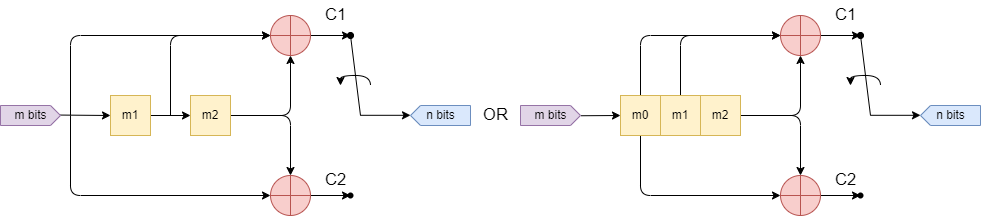
\includegraphics[width=\linewidth]{sections/pic/cosolythuyet/block_convolutional_encoder.png}
	\caption{Bộ mã hóa $(3, 1, 2)$.}
	\label{f_ex_block_conv_encoder}
\end{figure}

Trong đó, $C1 = m + m_1 + m_2$ và $C2 = m + m_2$.

\subsubsection{Ma trận sinh (Generator matrix)}

Sử dụng phương pháp biểu diễn mã chập bằng ma trận sinh, ta có thể lấy bộ mã hóa ở hình \ref{f_ex_block_conv_encoder} để thể hiện cách hoạt động của ma trận sinh. Từ hình \ref{f_ex_block_conv_encoder} ta có thể suy ra ma trận sinh $G$ là:
\[
\mathbf{G} = 
\begin{bmatrix}
	1 & 1 & 1 \\
	1 & 0 & 1 	
\end{bmatrix}
\]

Giả sử, $m_t = 1\text{, } m_{t - 1} = 0\text{, } m_{t - 2} = 1$, khi đó:
\[n = m \cdot G = \begin{bmatrix}
	m_t & m_{t - 1} & m_{t - 2}
\end{bmatrix} \cdot \begin{bmatrix}
	1 & 1 & 1 \\
	1 & 0 & 1 	
\end{bmatrix} = \begin{bmatrix}
	1 & 0 & 1
\end{bmatrix} \cdot \begin{bmatrix}
	1 & 1 & 1 \\
	1 & 0 & 1 	
\end{bmatrix} = \begin{bmatrix}
	0 & 0
\end{bmatrix}\]

\subsubsection{Sơ đồ lưới (Trellis Diagram)}

Sơ đồ trạng thái biểu diễn các trạng thái của thanh ghi và các chuyển tiếp giữa các trạng thái dựa trên bit đầu vào và bit đầu ra. Trong sơ đồ trạng thái, mỗi nút biểu diễn cho một trạng thái của thanh ghi. Các nội dung biểu diễn chuyển tiếp giữa các trạng thái, được gán nhãn bởi bit vào vầ bit đầu ra tương ứng. 

Để làm rõ hơn việc sử dụng sơ đồ trạng thái trong việc biểu diễn mã chập, ta sử dụng một bộ mã hóa chập ở hình \ref{f_ex_block_conv_encoder}. Với $K=3$ ta có tương ứng với 4 trạng thái là: \texttt{S0(00)}, \texttt{S1(01)}, \texttt{S2(10)}, \texttt{S3(11)}, và trạng thái chuyển tiếp có thể được tạo từ trạng thái này sang trạng thái khác, quá trình chuyển tiếp có thể là:

\begin{table}[H]
	\centering
	\begin{tabular}{|c|c|c|c|c|}
		\hline
		& \multicolumn{2}{c|}{Next State, if} & \multicolumn{2}{c|}{Output symbol, if} \\ \hline
		Current State & Input = 0 & Input = 1 & Input = 0 & Input = 1 \\ \hline
		S0 & S0 & S2 & 00 & 11 \\ \hline
		S1 & S0 & S2 & 11 & 00 \\ \hline
		S2 & S1 & S3 & 10 & 01 \\ \hline
		S3 & S1 & S3 & 01 & 10 \\ \hline
	\end{tabular}
	\caption{Bảng chuyển trạng thái của mã chập \( (3,1,2) \).}
	\label{t_fsm_conv_encoder}
\end{table}

Sơ đồ lưới là một mở rộng của sơ đồ trạng thái theo thời gian, biểu diễn tất cả các đường đi có thể của mã chập qua các bước thời gian. Sơ đồ lưới bao gồm các nút biểu diễn trạng thái tại mỗi bước thời gian. Các cung biểu diễn chuyển tiếp giữa các trạng thái, được gán nhãn bởi bit đầu vào và bit đầu ra.

Ở hình \ref{f_ex_block_conv_encoder}, ta có thể biểu diễn một cung chuyển tiếp đơn giản giữa hai đơn vị thời gian như sau:

\begin{figure}[H]
	\centering
	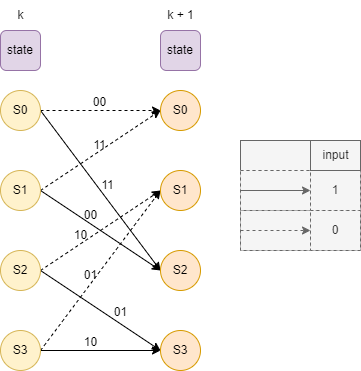
\includegraphics[width=.5\linewidth]{sections/pic/cosolythuyet/trellis-fsm-convolutional-code-coban.png}
	\caption{Sơ đồ lưới giữa hai đơn vị thời gian của bộ mã hóa $(3, 1, 2)$.}
	\label{f_trellis_unit_conv_encoder}
\end{figure}

Từ đó, ta có thể biểu diễn hoàn chỉnh cách biểu diễn bộ mã hóa chập bằng sơ đồ lưới như sau:

\begin{figure}[H]
	\centering
	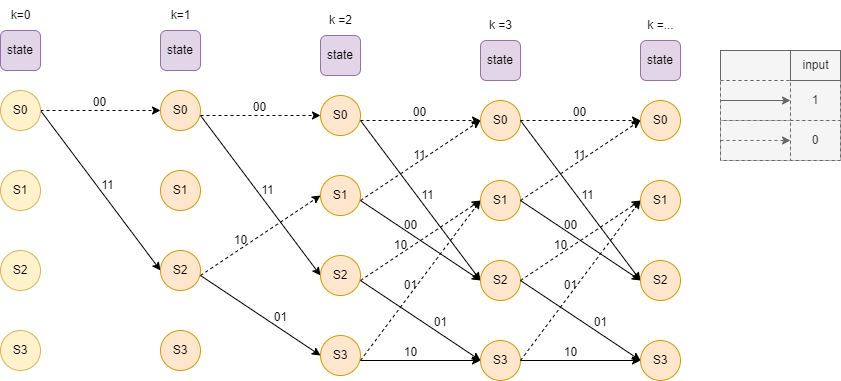
\includegraphics[width = \linewidth]{sections/pic/cosolythuyet/trellis-fsm-convolutional-code.png}
	\label{f_trellis_conv_encoder}
\end{figure}

Giả sử, chuỗi bit ngõ vào là \texttt{0101} thì ngõ ra tương ứng với chuỗi bit sau khi được mã hóa sẽ là \texttt{00 11 10 00}.

\subsection{Giải mã kênh truyền trong lĩnh vực truyền thông thông tin}

Giải mã kênh truyền là quá trình khôi phục thông tin gốc từ tín hiệu đã được mã hóa trên kênh truyền. Nó là bước ngược lại của quá trình mã hóa kênh, nhằm đưa dữ liệu về trạng thái ban đầu. Hiệu quả của giải mã kênh phụ thuộc vào nhiều yếu tố, bao gồm mô hình trạng thái và phương pháp giải mã được sử dụng. Mục tiêu chính là giảm thiểu lỗi trong quá trình truyền dữ liệu.

Ở hình \ref{f_mo-hinh-he-thong-truyen-thong-so} thể hiện hệ thống truyền thông đơn giản trong đó,

\begin{itemize}[label=-]
	\item Giải mã nguồn: khôi phục dữ liệu nguồn.
	\item Giải mã kênh: sửa lỗi do nhiễu trong quá trình truyền dẫn, đảm bảo dữ liệu nhận được gần nhất với dữ liệu gốc.
\end{itemize}

\subsection{Giải mã kênh truyền sửa dụng thuật toán Viterbi}

Thuật toán Viterbi là một giải pháp được sử dụng phổ biến để giải mã chuỗi bit được mã hóa bởi bộ mã hóa tích chập. Chi tiết của một bộ giải mã riêng phụ thuộc vào một bộ mã hóa tích chập tương ứng. Thuật toán Viterbi không phải là một thuật toán đơn lẻ có thể dùng để giải mã những chuỗi bit mà được mã hóa bởi bất cứ một bộ mã hóa chập nào.

Thuật toán Viterbi được khởi xướng bởi Andrew Viterbi vào năm 1967 như là một thuật toán giải mã cho mã chập qua các tuyến thông tin có nhiễu. Nó được sử dụng trong cả hai hệ thống CDMA và GSM, các modem số, vệ tinh, thông tin vũ trụ, và các hệ thống mạng cục bộ không dây. Hiện nay còn được sử dụng phổ biến trong kỹ thuật nhận dạng giọng nói, nhận dạng từ mã, ngôn ngữ học máy tính.

Thuật toán Giải mã Vitervi là một trong hai loại thuật toán giải mã được sử dụng với bộ mã hóa chập - là một loại giải mã tuần tự. Ưu điểm của giải mã tuần tự so với Viterbi là nó có thể hoạt động tốt với các mã chập có chiều dài ràng buộc lớn, nhưng nó lại có thời gian giải mã biến đổi.

Còn ưu điểm cảu thuật toán Giải mã Viterbi là nó có thời gian mã ổn định. Điều đó rất tốt cho việc thực thi bộ giải mã bằng phần cứng. Nhưng mà yêu cầu về sự tính toán của nó tăng theo hàm mũ như là một hàm của chiều dài rằng buộc. Vì vậy trong thực tế, người ta thường giới hạn chiều dài ràng buộc của nó là 9 ($k \leq 9$).

Thuật toán Viterbi là một giải pháp giải mã tối ưu cho các chuỗi bit được mã hóa bởi bộ mã hóa tích chập (convolutional encoder). Đây là thuật toán quyết định cứng (hard-decision) sử dụng nguyên lý quy hoạch động để tìm chuỗi trạng thái có xác suất cao nhất trong lưới trạng thái (trellis diagram).

\subsubsection*{Đặc điểm chính}
\begin{itemize}[label=-]
	\item \textbf{Tính tương thích}: Mỗi bộ giải mã Viterbi phải được thiết kế tương ứng với một bộ mã hóa tích chập cụ thể.
	
	\item \textbf{So sánh với giải mã tuần tự}:
	\begin{itemize}[label=+]
		\item Ưu điểm: Hiệu suất giải mã ổn định, độ phức tạp tính toán thấp
		\item Nhược điểm: Khó áp dụng cho mã có độ dài ràng buộc (constraint length) lớn
	\end{itemize}
	
	\item \textbf{Ứng dụng}:
	\begin{itemize}[label=+]
		\item Hệ thống thông tin di động (GSM, CDMA)
		\item Truyền dẫn vệ tinh
		\item Nhận dạng tiếng nói
	\end{itemize}
\end{itemize}

\subsubsection*{Nguyên lý hoạt động}
Thuật toán thực hiện các bước chính:
\begin{enumerate}
	\item Khởi tạo metric cho các trạng thái
	\item Tính toán độ tương đồng (branch metric)
	\item Cập nhật path metric
	\item Truy vết ngược (traceback) để tìm chuỗi giải mã tối ưu
\end{enumerate}

Phương trình cập nhật metric:
\[
\gamma_t(s',s) = \gamma_{t-1}(s') + \sum_{i=1}^n (r_i^{(t)} - c_i^{(t)})^2
\]
trong đó:
\begin{itemize}[label=-]
	\item $s', s$: các trạng thái liên tiếp
	\item $r_i^{(t)}$: bit nhận được tại thời điểm t
	\item $c_i^{(t)}$: bit mã hóa tương ứng
\end{itemize}

\subsection{Hard Decision và Soft Decision trong Giải Mã Mã Hóa Sửa Lỗi}

Trong các hệ thống thông tin số, mã hóa sửa lỗi (error-correction coding) đóng vai trò quan trọng trong việc đảm bảo dữ liệu được truyền qua kênh nhiễu một cách đáng tin cậy. Hai phương pháp giải mã phổ biến là \textbf{hard decision} và \textbf{soft decision}, được áp dụng cho cả mã khối (block codes) và mã chập (convolutional codes). Hard decision đơn giản hóa quá trình giải mã bằng cách đưa ra quyết định nhị phân, trong khi soft decision tận dụng thông tin xác suất để cải thiện hiệu suất. Phần tiếp theo sẽ trình bày cơ sở lý thuyết của hai phương pháp này \cite{Clark1981}.

\subsubsection{Hard decision (Quyết định cứng)}
Hard decision là phương pháp giải mã trong đó bộ giải mã nhận đầu vào dưới dạng các giá trị nhị phân (0 hoặc 1). Tại bộ giải điều chế (demodulator), tín hiệu nhận được sẽ được so sánh với một ngưỡng (threshold) để quyết định giá trị bit:

\begin{itemize}[label=-]
	\item Nếu tín hiệu vượt ngưỡng, bit được gán giá trị 1.
	\item Nếu tín hiệu dưới ngưỡng, bit được gán giá trị 0.
\end{itemize}
Quá trình này bỏ qua thông tin về độ tin cậy của tín hiệu, chỉ dựa vào quyết định cứng (hard decision).

Trong hard decision, bộ giải mã sử dụng khoảng cách Hamming (Hamming distance) để xác định chuỗi mã (codeword) gần nhất với chuỗi nhận được. Khoảng cách Hamming được định nghĩa là số vị trí mà hai chuỗi bit khác nhau. Ví dụ, với mã khối, thuật toán giải mã sẽ tìm chuỗi mã hợp lệ sao cho:
\[
d_H({r}, {c}) = \min_{{c} \in C} d_H({r}, {c}),
\]
trong đó $r$ là chuỗi nhận được, $c$ là chuỗi mã hợp lệ trong tập mã $C$, và $d_H$ là khoảng cách Hamming.

\textbf{Ưu và nhược điểm}

\begin{itemize}[label=-]
	\item Ưu điểm: Đơn giản, dễ triển khai trên phần cứng, yêu cầu tính toán thấp.
	\item Nhược điểm: Mất thông tin về độ tin cậy của tín hiệu, dẫn đến hiệu suất kém hơn trong kênh nhiễu mạnh, đặc biệt với các mã chập khi sử dụng thuật toán Viterbi.
\end{itemize}

\subsubsection{Soft decision (Quyết định mềm)}

Soft decision là phương pháp giải mã sử dụng thông tin xác suất hoặc giá trị liên tục từ bộ giải điều chế, thay vì quyết định nhị phân. Thay vì gán bit 0 hoặc 1, bộ giải mã nhận các giá trị thực (real-valued) đại diện cho độ tin cậy của mỗi bit. Phương pháp này tận dụng thông tin bổ sung để cải thiện khả năng sửa lỗi.

Trong soft decision, bộ giải mã thường sử dụng khoảng cách Euclidean (Euclidean distance) thay vì khoảng cách Hamming. Với chuỗi nhận được ${r} = (r_1, r_2, \ldots, r_n)$ và chuỗi mã ${c} = (c_1, c_2, \ldots, c_n)$, khoảng cách Euclidean được tính như sau:
\[
d_E({r}, {c}) = \sqrt{\sum_{i=1}^n (r_i - c_i)^2}.
\]
Bộ giải mã tìm chuỗi mã ${c}$ sao cho $d_E({r}, {c})$ là nhỏ nhất. Trong trường hợp mã chập, thuật toán Viterbi sử dụng soft decision bằng cách tính path metric dựa trên giá trị xác suất hoặc độ tin cậy của mỗi bit, thay vì chỉ đếm lỗi nhị phân.

\textbf{Ưu và nhược điểm}

\begin{itemize}[label=-]
	\item Ưu điểm: Cải thiện hiệu suất giải mã, đặc biệt trong kênh nhiễu Gaussian, nhờ sử dụng thông tin độ tin cậy. Hiệu suất có thể cải thiện 2–3 dB so với hard decision.
	\item Nhược điểm: Phức tạp hơn, yêu cầu tính toán cao hơn và bộ nhớ lớn hơn, đặc biệt khi triển khai trên phần cứng.
\end{itemize}

\subsubsection{So sánh Hard Decision và Soft Decision}

Hard decision và soft decision khác nhau ở cách xử lý đầu vào và độ phức tạp:
\begin{itemize}[label=-]
	\item Đầu vào: Hard decision chỉ nhận giá trị nhị phân, trong khi soft decision sử dụng giá trị liên tục hoặc xác suất.
	\item Hiệu suất: Soft decision thường vượt trội hơn trong môi trường nhiễu mạnh, đặc biệt với mã chập khi sử dụng thuật toán Viterbi.
	\item Độ phức tạp: Hard decision đơn giản hơn, phù hợp với các hệ thống có tài nguyên hạn chế, trong khi soft decision yêu cầu phần cứng mạnh hơn.
\end{itemize}

Cả hai phương pháp đều được sử dụng rộng rãi trong các hệ thống thông tin:
\begin{itemize}[label=-]
	\item Hard decision: Thường được dùng trong các hệ thống đơn giản như truyền dữ liệu tốc độ thấp hoặc khi tài nguyên phần cứng hạn chế.
	\item Soft decision: Được áp dụng trong các hệ thống hiện đại như truyền hình vệ tinh (DVB-S2), mạng không dây (Wi-Fi, LTE), và các hệ thống yêu cầu hiệu suất cao.
\end{itemize}
\end{document}